\documentclass[11pt,a4paper]{article}
\usepackage[T1]{fontenc}
\usepackage[utf8]{inputenc}
\usepackage{microtype}
\usepackage{amsmath,amssymb,amsfonts}
\usepackage{booktabs}
\usepackage{graphicx}
\usepackage{subcaption}
\usepackage{natbib}
\usepackage[colorlinks=true,linkcolor=blue,citecolor=blue,urlcolor=blue]{hyperref}
% cleveref errors if it is loaded before hyperref.
\usepackage[capitalize,noabbrev]{cleveref}

\title{Language-configured CEM on frozen LeWM (RTX 4090)}
\author{MMAGAI team\\Skoltech}
\date{}

\begin{document}
\maketitle

\begin{abstract}
This addendum runs cross-entropy planning with the frozen official LeWorldModel on a live Push-T environment.
The encoder is not finetuned, and text is not turned into a goal image.
An image-goal baseline on 50 episodes reaches the environment success test zero times.
A ridge probe of angle, used as the planning cost, reaches a scripted $+90^{\circ}$ target on 3 of 20 held-out starts and a $180^{\circ}$ target on none.
A latent skill head fit on 780 same-position turns beats a constant displacement and, when chased by CEM, usually leaves the block unturned.
\end{abstract}

\noindent\textbf{Keywords:}
LeWorldModel, Push-T, CEM, frozen encoder, language cost.

\section{Introduction}
\label{sec:intro}
The CPU probe already showed that block angle is linearly readable in the 192-dimensional LeWM latent, including after a half turn, so the encoder stays frozen \citep{maes2026lewm}.
A single vector $f(\mathrm{text})$ fit by least squares did not explain $\Delta z$.
This note asks whether that same frozen model can be used as a dynamics model for planning, first toward the environment's own goal image and then toward closed-set language commands.

\section{Methods}
\label{sec:methods}
The machine is a rented RTX 4090 with driver 535.309.01.
The run uses CPython 3.11.16 and PyTorch 2.5.1+cu121.
\texttt{torch.cuda.is\_available()} is true and the device name is NVIDIA GeForce RTX 4090.
The checkpoint is loaded with \texttt{load\_pretrained} on \texttt{quentinll/lewm-pusht} and moved to CUDA in eval mode.
Pixels follow the CPU sanity pipeline.
One frame encoded to shape $(1,1,192)$ in 0.068 seconds.
\texttt{eval.py} was not run, because it indexes the expert HDF5 set, which was not downloaded.
Planning is a live CEM: 300 samples, 30 iterations, 30 elites, horizon 5, and an action block of 5, for 50 environment steps.
The image-goal cost is the squared distance between the imagined terminal latent and the encoding of \texttt{info["goal"]}.
Eight live frameskip comparisons selected a global factor of 5 on environment actions before the action encoder.
The dataset's per-coordinate action normalizer was not available.
Probe-cost planning decodes $\hat\theta$ and $(\hat x,\hat y)$ from the imagined latent with ridge maps fit on the CPU train split.
The commands add $\pi/2$, $\pi$, or $-\pi/2$ to the current angle, or pull $(\hat x,\hat y)$ toward $(256,256)$.
The skill head is a two-layer MLP from $(z_t, e)$ to $\Delta z$, with $e$ a 4-way one-hot.
It is trained on 180 CPU train pairs and 600 new same-position turns collected on this GPU.
CEM then minimizes the squared gap between the imagined displacement and that head.
An energy network was not trained.

\section{Results}
\label{sec:results}
Image-goal CEM succeeds on 0 of 50 episodes.
Mean terminal position L2 is 300.07 and mean absolute angle error is 77.64 degrees.
The closest position L2 in the set is 28.95, above the success threshold of 20.
Wall time for the 50 episodes is 40.55 seconds.
Shorter prefixes of the same protocol, 10 and 20 episodes, were also 0 successes.
\Cref{tab:lang} compares the two language costs on the same 20 held-out scripted starts.
Probe-cost reach rate is 0.15 for ``rotate T 90'' and 0.00 for ``rotate T 180'' and ``rotate T -90''.
Mean xy error on those turns is 120.43, 108.37, and 95.24 pixels.
``put T on the target'' ends 86.44 pixels from $(256,256)$, with reach rate 0.00.
The skill head's final training batch MSE is 0.283.
On held-out pairs its mean residual L2 is 11.68 against a target mean L2 of 16.28.
Held-out pair MSE is 0.762.
When CEM chases the head, median absolute angle error is 90.00 degrees, 180.00 degrees, and 90.00 degrees for $+90^{\circ}$, $180^{\circ}$, and $-90^{\circ}$.
Those medians match the commanded offsets, so the block usually stays at the start angle.
Mean xy error under the skill head is 12.28, 27.29, and 16.18 pixels.
Reach rate is 0.00, 0.00, and 0.05.
``put T on the target'' is not measured for the skill head, because that command has no same-position pairs.
\Cref{fig:cmp} shows the mean angle errors.

\begin{table}[t]
\centering
\caption{Held-out language CEM.
Reach for a rotation is an angle error below 20 degrees.
The put row also requires xy error below 20 pixels.}
\label{tab:lang}
\begin{tabular}{llrrr}
\toprule
Cost & command & angle error & xy error & reach \\
\midrule
probe & rotate T 90 & 78.38 & 120.43 & 0.15 \\
probe & rotate T 180 & 119.70 & 108.37 & 0.00 \\
probe & rotate T $-90$ & 91.83 & 95.24 & 0.00 \\
probe & put T on the target & 73.23 & 86.44 & 0.00 \\
skill & rotate T 90 & 90.02 & 12.28 & 0.00 \\
skill & rotate T 180 & 169.97 & 27.29 & 0.00 \\
skill & rotate T $-90$ & 85.44 & 16.18 & 0.05 \\
\bottomrule
\end{tabular}
\end{table}

\begin{figure}[t]
\centering
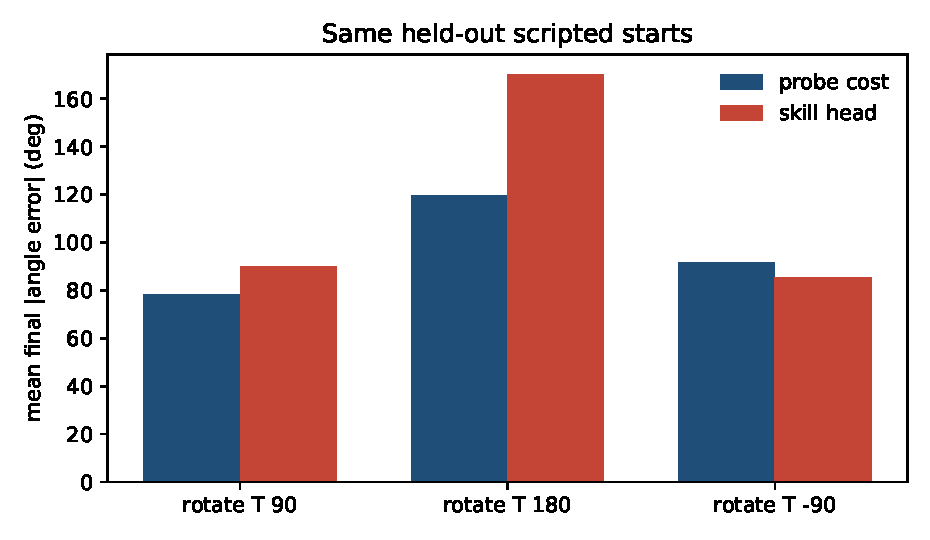
\includegraphics[width=0.86\linewidth]{figures_gpu/probe_vs_skill_angle.pdf}
\caption{Mean terminal absolute angle error on the same 20 starts.}
\label{fig:cmp}
\end{figure}

\section{Conclusion}
\label{sec:conclusion}
The encoder stays frozen.
A constant $\Delta z$ per command failed on the CPU, and the 4090 skill head only partially improves that fit.
Image-goal CEM did not solve live Push-T (0/50).
Probe-cost planning is the language port that sometimes hits $+90^{\circ}$.
Chasing $\mathrm{pred}_H$ does not turn the block on this protocol.

\bibliographystyle{plainnat}
\bibliography{refs}

\end{document}
